\subsection{Hamiltonian Systems}
Hamiltonian systems are quite analogous to gradient systems, at least in terms of definitions. Although they are a bit more general, we will restrict out attention to Hamiltonian systems on $\R^2$.
\begin{definition}[Hamiltonian systems]
A Hamiltonian system is a differential equation of the form 
$$x'' = - \nabla V(x)$$ 
where $V: D \to \R$ is a $C^2$ function.

Equivalently a system $z' = f(z)$ is Hamiltonian if there exists a map $H: D \to \R$ such that 
$$ x' = \frac{\partial H}{\partial y}(x, y), y' = -\frac{\partial H}{\partial x}(x, y) $$
\end{definition}

\noindent These are another class of systems where the Lyapunov function is easy to find. Namely we define
$$ L(x, y) = \frac{1}{2} |y|^2 + V(x) $$
(where $V$ is as in the first definition). Then if $(x(t), y(t))$ is a solution, we get
\begin{align*}
    \frac{d}{dt} L(x(t), y(t)) = y y' + \nabla V(x) x' = 0
\end{align*}
Thus we find that $L$ is actually constant along solutions. Since $L$ is continuous, if solutions get closer and closer together with time then they must have the same constant. To be precise, we have the following statement.

Suppose $\Gamma$ is a closed orbit that solves the equation and suppose $y \in D$ is such that $d(\Phi_t(y), \Gamma) \to 0$ as $t \to \infty$. Suppose $L|_{\Gamma} \equiv c_\Gamma$ and $L|_{\beta} \equiv c_\beta$ where $\beta$ is the orbit of $y$. Then continuity of $L$ implies that $c_\Gamma = c_{\beta}$.

\subsection{Wronskian}
The Wronskian is another tool that can be used to compare solutions of a differential equation (or even compare solutions of similar differential equations).
\begin{definition}[Wronskian]
Given two differentiable functions $f, g$ we define their Wronskian $W(f, g)$ to be a function where
$$ W(f, g)(x) = f(x) g'(x) - f'(x) g(x) = \det \matrix{f(x) & g(x)\\f'(x) & g'(x)} $$
\end{definition}

In order to see how useful this tool is, consider the equation
\begin{equation}\label{eq:second-order-normal}
    u''(x) + p(x) u'(x) + q(x) u(x) = 0 
\end{equation}
where $p(x)$ and $q(x)$ are some continuous functions. 
Clearly if $f, g$ are linearly dependent functions that $W(f, g) = 0$. However the converse also holds to some extent: if $f, g$ are linearly independent solutions to \autoref{eq:second-order-normal} then $W(f, g)$ is never 0. This fact allows for an easy proof of the following theorems.

\begin{theorem}[Sturm Separation Theorem]
Suppose $f, g$ are linearly independent solutions to \eqref{eq:second-order-normal}. Then $f$ must vanish between any two successive zeroes of $g$. In other words the zeroes of $f$ and $g$ occur alternately.
\end{theorem}
\begin{proof}
Let $a, b$ be 2 successive zeroes of $g$ with $a < b$. Suppose $g > 0$ on $(a, b)$. Then $g'(a) > 0$ and $g'(b) > 0$ (in principal we only have $g'(a) \geq 0$ rather than have the strict inequality. However if $g'(a) = 0$ then $W(f, g)(a) = 0$ which we know cannot happen. The same is true for $g'(b)$). Note that $W(f, g)(a) = f(a) g'(a)$ and $W(f, g)(b) = f(b) g'(b)$. Since $W(f, g)$ never vanishes, it must maintain its sign. Since $g'(a)$ and $g'(b)$ have opposing signs, the same must be true for $f(a)$ and $f(b)$. Then the Intermediate Value Theorem implies that $f$ is 0 somewhere on $(a, b)$ as desired. A symmetric argument holds if $g < 0$ on $(a, b)$.
\end{proof}
\begin{remark}
By noting that $\sin (kx)$ and $\cos (kx)$ are linearly independent solutions to $u'' + k^2 u = 0$, we find that their zeroes alternate (as we know them to).
\end{remark}

\begin{theorem}[Sturm Comparison Theorem]
Let $f(x)$ and $g(x)$ be non-trivial solutions to $u'' + p(x) u = 0$ and $v'' + q(x) = 0$ where $p(x) \geq q(x)$. Then $f(x)$ vanishes at least once between successive zeroes of $g$, unless $p(x) = q(x)$ and $f$ is a constant multiple of $g$.
\end{theorem}
\begin{proof}
Let $a < b$ be two successive zeroes of $g$ like before and suppose $f$ does not vanish on $(a, b)$. By replacing $f$ and/or $g$ with their negatives (those also satisfy the same ODE's), we can assume without loss of generality that $f, g$ are positive on $(a, b)$. As before, this means that $g'(a)$ is non-negative and $g'(b)$ is non-positive (because $f$ and $g$ no longer solve the same differential equation, we cannot use the same argument to conclude that the inequalities are strict). Thus what we find is that $W(f, g)(a) = f(a) g'(a) \geq 0$ and $W(f, g)(b) = f(b) g'(b) \leq 0$.

Then we compute that 
\begin{align*}
    \frac{d}{dx} W(f, g)(x) &= f' g' + f g'' - g' f' - g f''\\
    &= f(-qg) - (-pf)g\\
    &= (p - q) fg
\end{align*}
If $p \neq q$, then the above is positive on some neighbourhood so $W(f, g)$ is increasing on that neighbourhood (and remain non-decreasing outside it). But this contradicts $W(f, g)(b) \leq 0$ (since $W(f, g)(a) \geq 0$). Since we have covered the case with $p = q$ in the previous theorem, we are done. 
\end{proof}


\section{Limit Sets}
Limit sets are useful for understanding the ultimate behaviour of a given solution and thereby gaining insight into the limiting behaviour of the flow. 
\begin{definition}[Limit sets]
Given a solution $x(t)$ to the differential equation $x' = f(x)$ with $f: D \to \R^n$ (with $D \subset \R^n$ open), we define the $\omega$-limit set of $x$ as
$$ \omega(x) = \{ y \in D : \text{exists an increasing sequence $t_j$ to $\infty$ such that } \lim_{j \to \infty} x(t_j) = y \} $$
Equivalently we can write
$$ \omega(x) = \bigcap_{s > 0} \ol{\left\{x(t): t \geq s\right\}} $$

Analogously, we define the $\alpha$-limit set of $x$ as
$$ \alpha(x) = \{ y \in D : \text{exists a decreasing sequence $t_j$ to $-\infty$ such that } \lim_{j \to \infty} x(t_j) = y \} $$
or
$$ \alpha(x) = \bigcap_{s < 0} \ol{\{x(t): t \leq s\}} $$
\end{definition}
\begin{proposition}\label{prop:omega-equiv-def}
The two definitions of $\omega(x)$ (and $\alpha(x)$) are equivalent.
\end{proposition}
\begin{proof}
Clearly if there is an increasing sequence $t_j$ such that $x(t_j) \to y$ then $y$ is going to be in the closure of all $\{x(t): t \geq s\}$ (one could take this to be the definition of closure (in metric spaces)). Thus we wish to show inclusion in the other direction. This is also fairly easy to do. For every $j \in \N$, we find $t_j$ such that $t_j \geq j$ and $|y - x(t_j)| < \frac{1}{j}$ (both of these are possible by definition of the sets and the definition of closure). Then by construction $x(t_j) \to y$.
\end{proof}
\begin{remark}
For the second definition of $\omega(x)$, we could equivalently take $s \in \R$ or $s \in \N$ instead of $s > 0$. The same holds true for the second definition of $\alpha(x)$ (i.e. we could have $s \in \R$ or $s \in -\N$ instead of $s < 0$).
\end{remark}

Note that limit sets could be empty. For example if $x' = 1$, then we know solutions are of the form $x(t) = t + c$ and clearly both limit sets will be empty in this case. This is in fact typical of unbounded solutions or solutions that leave $D$. However, if $x(t)$ is a bounded solution that remains in $D$ for all $t > 0$, then $\omega(x)$ will be non-empty. This is easily seen by considering a compact set that contains $x(\R^+)$ and verifying that the \href{https://en.wikipedia.org/wiki/Finite_intersection_property#Applications}{finite intersection property} holds for the family of sets in the (second) definition of $\omega(x)$. An entirely analogous argument holds for $\alpha(x)$.

\subsection{Examples}
Consider \autoref{fig:limit-set-eg1}. In this case we have $\omega(x) = \left\{p\right\}$ and $\alpha(x) = \left\{q\right\}$. The situation is reversed for $y(t)$, namely we have $\omega(x) = \left\{q\right\}$ and $\alpha(x) = \left\{p\right\}$. Such solutions that connect different equilibrium points to one another are called heteroclinic solutions. Solutions that connect the same equilibria are called homoclinic.

We see that $z(t)$ has a closed orbit so, in fact, we get $\omega(z) = \alpha(z) = \left\{ z(t): t \in \R \right\}$. Finally we have $r(t)$ with $\omega(r) = \left\{z(t): t \in \R \right\}$ and $\alpha(r) = \left\{a\right\}$.
\begin{figure}[h]
    \centering
    \includegraphics[scale=0.5]{Images/limit_set_eg1.png}
    \caption{Example of limit sets, assume $p, q, a$ are equilibria}
    \label{fig:limit-set-eg1}
\end{figure}
Finally \autoref{fig:limit-set-eg2} highlights another case that may occur with $\omega(w) = \left\{x(t): t \in \R \right\} \cup \left\{y(t): t \in \R \right\}$ and $\alpha(w) = \left\{a\right\}$. Roughly speaking, these examples illustrate what all limit sets in the plane look like.

\begin{figure}[h]
    \centering
    \includegraphics[scale=0.5]{Images/limit_set_eg2.png}
    \caption{Example of limit sets, assume $p, q, a$ are equilibria}
    \label{fig:limit-set-eg2}
\end{figure}


Limit sets have some nice properties as well. 
\begin{proposition}\label{prop:omega-properties}
Suppose $x(t)$ be a bounded solution to $x' = f(x)$ and let $\omega(x)$ denote the $\omega$-limit set of $x$. If $y \in \omega(x)$, then $y(\R) \subset \omega(x)$. Moreover $\omega(x)$ is connected.
\end{proposition}
\begin{remark}
The above properties are also held by $\alpha$-limit sets. This can be verified by tweaking the proofs below where appropriate (in the obvious manner) or realising that $\alpha(x)$ is the $\omega-$limit set of the solution to $x' = -f(x)$.
\end{remark}
\begin{proof}
Suppose $y \in \omega(x)$ and let $t \in \R$ be arbitrary. Then there exists an increasing $t_j$ to infinity such that $\lim_{j \to \infty} x(t_j) = y$. Then
$$ \Phi_t(y) = \lim_{j \to \infty} \Phi_t(x(t_j)) = \lim_{j \to \infty} x(t_j + t) $$
where the final term is an element of $\omega(x)$ by definition.

We can prove this using the second definition of $\omega(x)$ as well.
\begin{align*}
    \Phi_t(\omega(x)) &= \Phi_t \left( \bigcap_{s > 0} \ol{\{x(r): r \geq s\}} \right)\\
    &\subset \bigcap_{s > 0} \Phi_t (\ol{\{x(r) : r \geq s\}})\\
    &\subset \bigcap_{s > 0} \ol{ \Phi_t(\{x(r): r \geq s\}) }\\
    &\subset \bigcap_{s > 0} \ol{\{x(t + r): r \geq s\}}\\
    &= \omega(x)
\end{align*}

Recall that a closed set $C \subset \R^n$ is connected if for any partition $C = C_1 \cup C_2$ where $C_1, C_2$ are closed with $C_1 \cap C_2 \neq \emptyset$ we have that $C_1 = \emptyset$ or $C_2 = \emptyset$.

Now suppose $\omega(x)$ is not connected. Let $C_1, C_2$ form a partition of $\omega(x)$. In other words $C_1, C_2$ are both disjoint, non-empty closed sets whose union is equal to $\omega(x)$. Let $y_1 \in C_1$ and $y_2 \in C_2$. Note that $C_1$ and $C_2$ are bounded as well and are thus compact. Thus there exists $m > 0$ such that $|z_1 - z_2| \geq m$ for all $z_1, z2 \in C_1, C_2$ respectively. By definition of $\omega(x)$, we know there exist increasing sequences $s_j$ and $t_j$ such that $\lim_{j \to \infty} x(s_j) = y_1$ and $\lim_{j \to \infty} x(t_j) = y_2$.  Without loss of generality we can assume that $s_j < t_j$ for all $j$. Consider the construction of the sequences in \autoref{prop:omega-equiv-def}. We first construct the $s_j$, then when constructing the second sequence, we just always ensure to choose $t_j$ to be larger than $s_j$.

Consider the map on $[s_j, t_j]$ (for every $j$) where we map $r$ in this open interval to $d(x(r), C_1)$ (note that this distance function is well-defined since $C_1$ is closed and even compact). We see that $d(x(s_j), C_1) = 0$ and $d(x(t_j), C_1) \geq m$. Thus my the Intermediate Value Theorem, there exists some $r_j \in (s_j, t_j)$ such that $d(x(r_j), C_1) \geq \frac{m}{2}$. Similarly, we can argue that $r_j$ are such that $d(x(r_j), C_2) \geq \frac{m}{2}$ (in fact there needs to be a slight argument for why we can pick the same $r_j$ to satisfy both inequalities. It's not a terribly difficult argument but is besides the point. Quite frankly all we need is that $x(r_j)$ is some positive distance from both $C_1$ and $C_2$ and clearly this can be done). We now have another increasing sequence $r_j$ so we must have $p := \lim_{j \to \infty} x(r_j) \in \omega(x)$ (if the limit does not exist, we can always pass to a convergent subsequence by sequential compactness). But $p$ cannot be in either of $C_1$ or $C_2$ since it is a positive distance away from both (follows from the fact that the map defined above on $[s_j, t_j]$ is actually continuous). This contradicts $\omega(x) = C_1 \cup C_2$.
\end{proof}

\subsection{Poincaré-Bendixson Theorem}

In general, limit sets can be pretty messy. However, on the plane limit sets are (relatively) well-behaved. In fact, we have the Poincaré-Bendixson (not a typo) theorem, which roughly says that $\omega(x)$ will either contain equilibrium points or will be a periodic solution to the differential equation. Before we prove this statement (or even state it precisely), a definition.

\begin{definition}
A section $\gamma$ for the flow of $x' = f(x)$ is a curve segment (i.e. a continuous map on $\R$) such that it intersects the vector field transversally. That is $\det(\gamma'(s), f(\gamma(s))) \neq 0$ (where each entry is the column in the matrix).
\end{definition}
Note that $\gamma'(s)$ tells us the ``direction'' of the section at $\gamma(s)$ (the push forward of the tangent vector at $s$ if you want) and $f(\gamma(s))$ is the vector field at $\gamma(s)$ so if the determinant is non-zero, we know the two vectors are linearly independent, giving the transversal intersection of $\gamma$ with the vector field. In fact by reversing the parameterisation of $\gamma$ if necessary, you can always assume the determinant to be positive.

\begin{theorem}[Poincaré-Bendixson]
Let $f: D \subset \R^2 \to \R^2$ be $C^1$ and $x(t)$ a solution to $x' = f(x)$ that is contained entirely in $D$. Suppose that $\omega(x)$ contains no equilibrium points and is contained in a compact set. Then $\omega(x)$ is a periodic solution to the ODE. In other words, there is some $\tau > 0$, such that $y(t) = y(t + \tau)$ for all $t$. Moreover, we have that $\omega(x) = \left\{y(t) : 0 \leq t \leq \tau\right\}$.
\end{theorem}
\begin{proof}
Let $y \in \omega(x)$. Since $\omega(x)$ does not contain any equilibria we know that that $f(y) \neq 0$. Then by continuity of $f$, we can find a small section through $y$ on which $f$ is non-zero (in fact if we take $\gamma$ to be small enough then the vector field is going to be roughly parallel on the section). The first part of this proof is roughly about understanding how solutions of the ODE behave, where the section $\gamma$ will be a very useful tool for doing so. To be a bit more precise, we will see that if a solution intersects a section multiple times, then it must do so in a very particular way. We will then find a section which $y$ will intersect repeatedly but then argue that this is always through the same point (curiously, it's only this last point that will require the fact that $y \in \omega(x)$). This will allow us to conclude that the orbit of $y$ is periodic and contained in $\omega(x)$. Finally we will show that this inclusion is in fact an equality.

Now suppose $\tilde{x}(t)$ is any solution to the ODE that intersects the section $\gamma$ at times $t_1, t_2, t_3, \dots$ with $t_i < t_{i + 1}$. That is there are some $s_1, s_2, s_3, \dots$ such that $\tilde{x}(t_1) = \gamma(s_1), \tilde{x}(t_2) = \gamma(s_2), \dots$. Then we claim that $s_i < s_{i + 1}$ for all $i$ or $s_i > s_{i + 1}$ for all $i$ (in other words either $s_1 < s_2 < s_3 < \dots$ or $s_1 > s_2 > s_3 > \dots$). In order to verify this consider \autoref{fig:section-monotone}.

\begin{figure}[h]
    \centering
    \includegraphics[scale=0.8]{Images/section_monotone.png}
    \caption{Solutions are trapped inside $C$ after entering it}
    \label{fig:section-monotone}
\end{figure}

Let $C$ be the region bounded by $\left\{\tilde{x}(t): t \in [t_1, t_2]\right\} \cup S$ where $S$ is the portion of the section that is between $\tilde{x}(t_1)$ and $\tilde{x}(t_2)$ (in other words $S = \left\{\gamma(s) : s \in [s_2, s_1]\right\}$ assuming $s_2 < s_1$ as in the figure). It is clear that the region $C$ is positively invariant: solutions cannot exit by crossing the solution curve $x$ since this would violate uniqueness and they cannot exit via $S$ since the vector field is pointing into $C$ (this also highlights why it's important that we're in the plane, clearly the argument above breaks down for higher dimensions). Thus if $\tilde{x}(t)$ intersects $\gamma$ again at $\gamma(s_3)$, it must do so inside $C$ implying that $s_3 < s_2$. There remain 3 other cases to consider (1 other if we ignore mirror images) and the arguments for all other cases are near identical.
\begin{figure}[h]
    \centering
    \includegraphics[scale=0.7]{Images/section_monotone_other_cases.png}
    \caption{Other cases for showing monotonicity. Note in the second two cases it is the `complement' of $C$ that is positively invariant.}
    \label{fig:section-monotone-other-cases}
\end{figure}

We now have some understanding of how solutions behave if they intersect a section multiple times. We are interested in the solution that passes through $y$. So in order to study it further, let us try and find a section that this solution (the one through $y$) will intersect repeatedly.

Let $z \in \omega(y)$ and let $\tilde{\gamma}$ be a section through $z$ (note how we are using sections and limit sets to understand the behaviour of the solution through $y$. Hopefully this serves as motivation for why these are useful tools). We define a map $h: \R^2 \to \R^2$ by $h(s, t) = \Phi_t(\tilde{\gamma}(s))$. In other words, we use the first coordinate to say where on the section we are and the second coordinate to say how far forward (or backward) we evolve in time. Note that 
$$ \frac{\partial h}{\partial s} = \Phi_t'(\tilde{\gamma}(s)) \tilde{\gamma}'(s), \frac{\partial h}{\partial t} = f(\Phi_t(\tilde{\gamma}(s))) $$
This means that
$$ Dh(0, 0) = \matrix{\tilde{\gamma}'(0) & f(\tilde{\gamma}(0))} $$
which, by construction of $\tilde{\gamma}$, is invertible. Thus we can apply the Inverse Function Theorem to conclude that $h$ is at least locally a homeomorphism (and in fact this holds for every point $(s, 0)$ since $\Phi_0$ is always the identity). 

Let $V$ be the neighbourhood of $z$ upon which $h$ acts homeomorphically. Since $y(t_n) \to z$, we can easily pick $t_n$ such that $y(t_n) \in V$. By applying the inverse of $h$, we find there is some $(s, t)$ near the origin such that $h(s, t) = \Phi_{t}(\tilde{\gamma}(s)) = y(t_n)$. This means that $\Phi_{-t}(y(t_n)) = \Phi_{-t}(\Phi_{t}(\tilde{\gamma}(s))) = \tilde{\gamma}(s)$ which of course lies on the section. Since $\Phi_{-t}(y(t_n)) = y(t_n - t)$ we see that the solution through $y$ intersects $\tilde{\gamma}$ (geometrically what we're doing is finding a neighbourhood of the section where flow is essentially parallel. We find $y(t_n)$ is in this neighbourhood and then flow it forward or backward until it reaches the section). By repeating this for all other $y(t_n)$ which lie in $V$, of which there are infinitely many, we see that $y(t)$ intersects this section infinitely many times. All that remains to show is that all of these points are in fact the same.\footnote{Note that we are only trying to find a section that the solution through $y$ intersects repeatedly. Since $x$ intersects $\gamma$, the original section, repeatedly and $x(t_n)$ is close to $y$, one would hope that you can show that $y$ must intersect $\gamma$ repeatedly as well (so we wouldn't have to look at another section to make the above argument). Unfortunately it's not clear to me how to make this argument, but perhaps you, my dear reader, are clever enough to think of something.}\\

The claim is as follows: if a solution through $y$ where $y \in \omega(x)$ intersects a section multiple times, then it must do so at the same point each time. Suppose not. In other words, suppose $y_1$ and $y_2$ are distinct points on the solution through $y$ that also lie on the section $\tilde{\gamma}$. Like in the previous paragraph, we find neighbourhoods $V_1, V_2$ of $y_1$ and $y_2$ respectively where the homeomorphisms can be found and without loss of generality we can assume that these are disjoint (simply consider smaller neighbourhoods if not). The intersections of $V_1$ and $V_2$ with the section $\tilde{\gamma}$ are going to form sections of their own. By using the homeomorphisms as in the previous case if necessary, we can assume that $x(t_n)$ intersect $\tilde{\gamma}$ for all (sufficiently large) $n$. Thus $x$ must intersect the entire section $\tilde{\gamma}$ as well as the smaller, disjoint sections monotonically in all cases. Clearly this cannot be done, see \autoref{fig:unique-intersection}.

\begin{figure}[h]
    \centering
    \includegraphics[scale=0.4]{Images/unique_intersection.png}
    \caption{$x(t_n)$ must eventually be in the top box but this breaks monotonicity on $\gamma$}
    \label{fig:unique-intersection}
\end{figure}

Thus all the intersections pass through the same point which immediately implies (by uniqueness) that the solution through $y$ is periodic. By \autoref{prop:omega-properties}, we know that the orbit of $y$ is contained in $\omega(x)$. What remains to show is that this is in fact the entirety of $\omega(x)$. In fact there is a slightly more general statement that holds. If $\omega(x)$ contains a closed orbit $\Gamma$, then $\omega(x) = \Gamma$.\\

We will show that $d(\Phi_t(x), \Gamma) \to 0$ as $t \to \infty$. 
By everything we have done thus far, we know there exists an increasing sequence $t_n$ such that $\Phi_{t_n}(x) \in \gamma$, $\Phi_{t_n}(x) \to y$ and $\Phi_{t}(x) \notin \gamma$ if $t_{n} < t < t_{n + 1}$. We will use $\Gamma$ to denote the orbit of $y$ where $y \in \omega(x)$ as before.

By definition, we know that $x_n := x(t_n)$ come arbitrary close $y$, so we would like to say the distance between $\Phi_t(x(t_n))$ and $\Phi_t(y)$ is pretty small.\footnote{Side note: $\Phi_t(x(t_n)) = \Phi_{t_n + t}(x)$. So by renaming variables, the statement above is equivalent to saying that $\Phi_{t - t_n}(x_n)$ is close to $\Phi_{t- t_n}(y)$. This is not terribly important but we will use this at the very end so hopefully it won't seem too mysterious. } We know for any fixed $t$, we could prove this rigorously using continuous dependence on initial conditions (for example we know that solutions can only differ by some exponential amount as time evolves. Unfortunately, this bound is not uniform; it depends on $t$). This is where we use the fact that the solution through $y$ is periodic, say with period $\tau$. Since the $x_n$ are pretty close to $y$, they should also be roughly periodic with a period of about $\tau$. In fact this is exactly what is captured by the choice of $t_n$: these are the times when the solution $x$ comes back to the section (and since the $x(t_n)$ converge we know that $x(t_{n + 1})$ is close $x(t_{n})$ which illustrates the `rough periodicity'). Since $y$ has period $\tau$, we should expect that $t_{n + 1}$ and $t_{n}$ differ by about $\tau$ as well. But notice how we are basically done now: any $t$ is going to lie between some $t_n$ and $t_{n + 1}$ so we only ever need to evolve by $\tau$ (or whatever the largest difference between all the $t_{n + 1}$ and $t_n$ is). Since we have a maximal time interval to look at, we can use continuous dependence to determine how close the initial point needs to be to $y$ in order to ensure we remain close to $y$ for all time in this interval. After evolving $x_n$ by this amount (at most), we will be even closer to $y$, so continuous dependence will still hold! Now all that remains to do is turn the above into precise mathematics (buckle up?).

As is typical in math proofs, we will work backwards. First we find the bound for $t_{n + 1} - t_n$. Let $V$ be a neighbourhood of $y$ such that we have the homeomorphism $h$ from previous paragraph(s) on it. Let $\epsilon$ such that a closed rectangle of height $2 \epsilon$ centered on the $x$-axis and is contained in $h^{-1}(V)$ (in other words $\epsilon$ is such that $J \times [-\epsilon, \epsilon]$ is contained in $h^{-1}(V)$ where $J$ is some closed interval itself). Let $V_{\epsilon}$ be the image of this rectangle under $h$. Since $\Phi_\tau(y) = y \in V_\epsilon$ (we take the closed interval $J$ appropriately so $y$ remains in $V_\epsilon$), we know that for $x_n$ sufficiently large we will have $\Phi_\tau(x_n) \in V_\epsilon$. Therefore $\Phi_{\tau + t}(x_n) \in \gamma$ for some $t \in [-\epsilon, \epsilon]$. Since the $t_n$ are chosen so that successive ones intersect $\gamma$ while everything between $t_{n}$ and $t_{n + 1}$ doesn't, we find that $t_{n + 1} - t_n \leq \tau + \epsilon$. 

Now we have a bound for $t_{n + 1} - t_n$. From here, as outlined above, the procedure is quite simple. Suppose $\beta > 0$ is given. By continuous dependence there exists some $\delta$ such that $\left|z - y\right| < \delta$ implies that $\left| \Phi_{t}(z) - \Phi_t(y) \right| < \beta$. Moreover, we can choose $\delta$ so that this holds for all $t$ where $|t| \leq \tau + \epsilon$ (I turn especially to \autoref{thm:sim-init-conds}. We are working with a $C^1$ function on a compact set so we know it is Lipschitz and we're working in the simpler case with $\epsilon_1 = \epsilon_2 = 0$). Since the $x_n$ converge to $y$, we find some $n_0$ such that $|y - x_n| < \delta$ for all $n \geq n_0$. Then for $t \geq t_{n_0}$ we find $n$ such that
$$ t_n \leq t < t_{n + 1} $$
With this $n$, we find that
\begin{align*}
    d(\Phi_{t}(x), \Gamma) &\leq \left| \Phi_t(x) - \Phi_{t - t_n}(y) \right|\\
    &= \left| \Phi_{t - t_n}(x_n) - \Phi_{t - t_n}(y) \right|\\
    &< \beta
\end{align*}
Here we use the fact that $t - t_n \leq \tau + \epsilon$. Thus by taking $t$ to be sufficiently large, we can make $d(\Phi_t(x), \Gamma)$ arbitrarily small, finally, \textit{finally}, proving the theorem.
\end{proof}

I apologise, the previous proof should probably have been split into multiple lemmas. But then again, if I was good at making decisions, this wouldn't exist so :)
